% Vista preliminar del c�digo fuente

%% LyX 2.0.3 created this file.  For more info, see http://www.lyx.org/.
% Vista preliminar del c�digo fuente

%% LyX 2.0.3 created this file.  For more info, see http://www.lyx.org/.
%% Do not edit unless you really know what you are doing.
\documentclass[spanish]{article}
%\usepackage[T1]{fontenc}
\usepackage[latin9]{inputenc}
\usepackage{geometry}
\geometry{verbose,tmargin=2cm,bmargin=2cm,lmargin=2cm,rmargin=2cm}
\usepackage{fixltx2e}
\usepackage{babel}
\usepackage{amsmath}
\usepackage[pdftex]{graphicx} % LaTeX
\DeclareGraphicsExtensions{.bmp,.png,.pdf,.jpg}
%\usepackage{graphicx} % Soporte para gr�ficos
\usepackage{float}
\usepackage{color}
\addto\shorthandsspanish{\spanishdeactivate{~<>}}

\begin{document}
\selectlanguage{spanish}%

\begin{minipage}[c]{.49\linewidth}
\textbf{\large Pontificia Universidad Javeriana de Cali}{\large \par}
\textbf{\large Departamento de Econom�a}{\large \par}
\textbf{\large Econometr�a I}{\large \par}
\textbf{\large Profesor: Orlando Joaqui Barandica}{\large \par}
\end{minipage}\hfill
\begin{minipage}[b]{.4\linewidth}
    
\includegraphics[width=1\textwidth]{Imagen1.JPG}
\end{minipage}


\vspace{1cc}


\begin{center}
\textbf{\large Parcial 1}
\par\end{center}{\large \par}

\vspace{1cc}

\textbf{Nombre:}$\_\_\_\_\_\_\_\_\_\_\_\_\_\_\_\_\_\_\_\_\_\_\_\_\_\_\_\_\_\_\_\_\_\_\_\_\_\_\_\_\_\_\_\_\_\_\_\_\_ $

\vspace{1cc}

\parbox[c]{0.98\linewidth}{\textit{\textbf{Nota:} Se dispone de 120 minutos para la soluci�n del examen. Registre su nombre y c�digo en su hoja de respuesta.}} \\

%\vspace{0.5cm}


\begin{enumerate}

%%%%%%%%%%%%%%%%%%%%%%%%%%%%%%%%%%%%Punto 1

\item \textbf{[10 Puntos]} De una muestra de 10 observaciones se obtuvieron los siguientes resultados

\begin{equation}
\sum Y_i=1110 \quad \sum X_i=1700 \quad \sum{X_iY}_i=205500 \quad \sum X_i^2=322000 \quad \sum X_i^2=322000 \quad \sum Y_i^2=132100 \nonumber
\end{equation}


con el coeficiente de correlaci�n $r = 0.9758$. Pero al verificar estos c�lculos se descubri� que se registraron dos pares de observaciones:

\begin{center}
(Y,X)=(90, 120) \\
(Y,X)=(140, 220)

en lugar de

(Y,X)=(80, 110) \\
(Y,X)=(150, 210)
\end{center}



Cu�l ser� el efecto de este error en $r$?. Obtenga la $r$ correcta.


\item \textbf{[10 Puntos]} Se ha realizado un an�lisis de regresi�n para evaluar la relaci�n entre el PIB per c�pita en miles d�lares (X) y el gasto social en salud en miles de d�lares (Y) en una muestra de 32 pa�ses. Los resultados del an�lisis de regresi�n incluyen un coeficiente de determinaci�n de 0.75 y un coeficiente de correlaci�n de -0.8676.


\begin{center}
\begin{tabular}{|c|c|c|}
\hline 
Variable & Promedio & Varianza \\ 
\hline 
PIB per c�pita & 3.2172 & 0.9573 \\ 
\hline 
Gasto social en salud & 20.0906 & 36.3241 \\ 
\hline 
\end{tabular} 
\end{center}

\begin{figure}[h!]
\begin{center}
    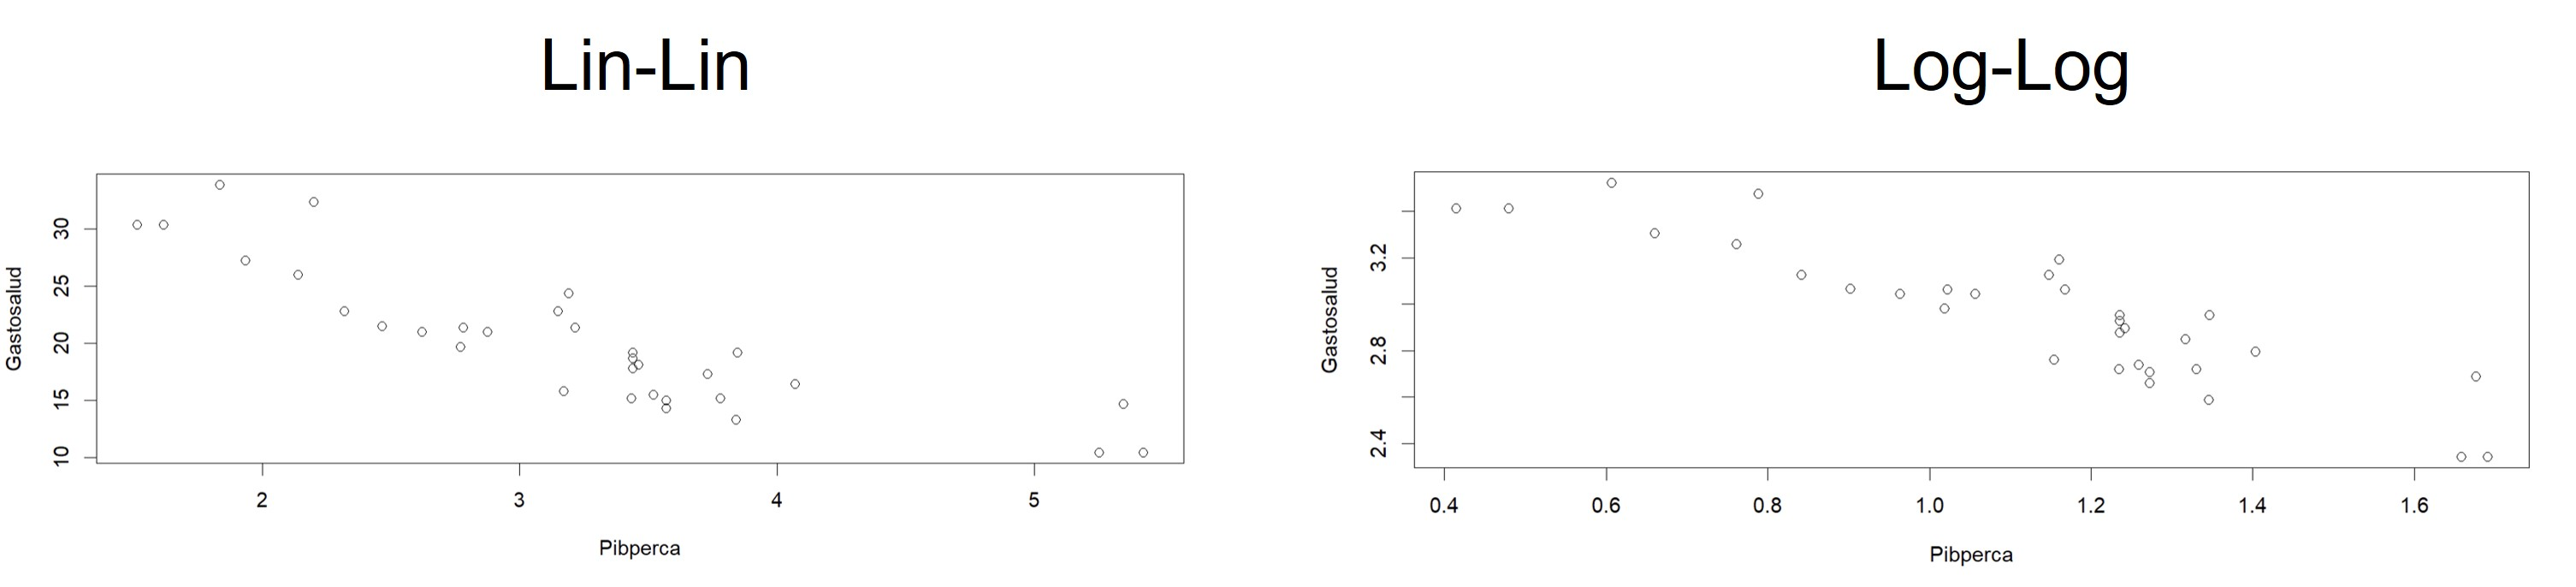
\includegraphics[width=0.90\textwidth]{Imagen2.JPG}
\end{center}
\end{figure}

\begin{enumerate}
\item �Cu�l es la ecuaci�n de la l�nea de regresi�n?
\item Suponga que ahora se quiere estimar el modelo con las unidades de las variables en millones de d�lares, �Cu�l es la ecuaci�n de la l�nea de regresi�n?
\item Si se aplica una transformacion Log-Log sobre el modelo, el coeficiente de determinaci�n disminuye o aumenta. En este caso espec�fico seg�n el gr�fico. Argumente.

\end{enumerate}


\item \textbf{[10 Puntos]} Use la base de datos WAGE2 de la librer�a de Wooldridge para estimar una regresi�n simple que explique el salario mensual (wage) en t�rminos de la puntuaci�n del coeficiente intelectual (IQ).

\begin{verbatim}
En R:
library(wooldridge)
data(wage2)
\end{verbatim}

\begin{enumerate}
\item Es la variable IQ significativa para explicar el salario?
\item Que interpretan los estimadores de $\hat{\beta_0}$ y $\hat{\beta_1}$?
\item Interprete el $R^2$
\end{enumerate}



\item \textbf{[10 Puntos]} 	En la regresi�n $Y_i= \beta_0+\beta_1X+u$ suponga que se multiplica cada valor de $X$ por una constante, $7$, por ejemplo. �Cambiar� esto los residuos y los valores ajustados de $Y$ ? Explique. �Qu� sucede si se agrega un valor constante, por ejemplo, $7$, a cada valor de $X$? Demuestre.



\item \textbf{[10 Puntos]} Se ha estimado el siguiente modelo $Y_i= \beta_0+\beta_1X_i+u_i$ con una muestra de 935 observaciones, de tal manera que la tabla anova es la que sigue a continuaci�n.

\begin{center}
\begin{tabular}{|c|c|c|c|c|c|}
\hline 
Fuente Var. & Suma de Cuadr. & gl & Cuadrados Med. & F & pvalue\\ 
\hline 
Modelo & 14589783 & 1 & 14589783 &  & 2.2e-16 \\ 
\hline 
Error & 138126386 &  &  &  & \\ 
\hline 
Total &  &  &  &   & \\ 
\hline 
\end{tabular} 
\end{center}


\begin{enumerate}
\item Complete la tabla
\item Con base en esta informaci�n podemos asegurar que $X$ tiene un efecto significativamente lineal sobre $Y$
\item Calcule $R^2$
\end{enumerate}






\end{enumerate}


\end{document}